\documentclass[a4paper, 14pt]{extarticle}

% Поля
%--------------------------------------
\usepackage{geometry}
\geometry{a4paper,tmargin=2cm,bmargin=2cm,lmargin=3cm,rmargin=1cm}
%--------------------------------------


%Russian-specific packages
%--------------------------------------
\usepackage[T2A]{fontenc}
\usepackage[utf8]{inputenc} 
\usepackage[english, main=russian]{babel}
%--------------------------------------

\usepackage{textcomp}

% Красная строка
%--------------------------------------
\usepackage{indentfirst}               
%--------------------------------------             


%Graphics
%--------------------------------------
\usepackage{graphicx}
\graphicspath{ {./images/} }
\usepackage{wrapfig}
%--------------------------------------

% Полуторный интервал
%--------------------------------------
\linespread{1.3}                    
%--------------------------------------

%Выравнивание и переносы
%--------------------------------------
% Избавляемся от переполнений
\sloppy
% Запрещаем разрыв страницы после первой строки абзаца
\clubpenalty=10000
% Запрещаем разрыв страницы после последней строки абзаца
\widowpenalty=10000
%--------------------------------------

%Списки
\usepackage{enumitem}

%Подписи
\usepackage{caption} 

%Гиперссылки
\usepackage{hyperref}

\hypersetup {
	unicode=true
}

%Рисунки
%--------------------------------------
\DeclareCaptionLabelSeparator*{emdash}{~--- }
\captionsetup[figure]{labelsep=emdash,font=onehalfspacing,position=bottom}
%--------------------------------------

\usepackage{tempora}

%Листинги
%--------------------------------------
\usepackage{listings}
\lstset{
  basicstyle=\ttfamily\footnotesize, 
  %basicstyle=\footnotesize\AnkaCoder,        % the size of the fonts that are used for the code
  breakatwhitespace=false,         % sets if automatic breaks shoulbd only happen at whitespace
  breaklines=true,                 % sets automatic line breaking
  captionpos=t,                    % sets the caption-position to bottom
  inputencoding=utf8,
  frame=single,                    % adds a frame around the code
  keepspaces=true,                 % keeps spaces in text, useful for keeping indentation of code (possibly needs columns=flexible)
  keywordstyle=\bf,       % keyword style
  numbers=left,                    % where to put the line-numbers; possible values are (none, left, right)
  numbersep=5pt,                   % how far the line-numbers are from the code
  xleftmargin=25pt,
  xrightmargin=25pt,
  showspaces=false,                % show spaces everywhere adding particular underscores; it overrides 'showstringspaces'
  showstringspaces=false,          % underline spaces within strings only
  showtabs=false,                  % show tabs within strings adding particular underscores
  stepnumber=1,                    % the step between two line-numbers. If it's 1, each line will be numbered
  tabsize=2,                       % sets default tabsize to 8 spaces
  title=\lstname                   % show the filename of files included with \lstinputlisting; also try caption instead of title
}
%--------------------------------------

%%% Математические пакеты %%%
%--------------------------------------
\usepackage{amsthm,amsfonts,amsmath,amssymb,amscd}  % Математические дополнения от AMS
\usepackage{mathtools}                              % Добавляет окружение multlined
\usepackage[perpage]{footmisc}
%--------------------------------------

%--------------------------------------
%			НАЧАЛО ДОКУМЕНТА
%--------------------------------------

\begin{document}

%--------------------------------------
%			ТИТУЛЬНЫЙ ЛИСТ
%--------------------------------------
\begin{titlepage}
\thispagestyle{empty}
\newpage


%Шапка титульного листа
%--------------------------------------
\vspace*{-60pt}
\hspace{-65pt}
\begin{minipage}{0.3\textwidth}
\hspace*{-20pt}\centering

\includegraphics[width=\textwidth]{emblem}
\end{minipage}
\begin{minipage}{0.67\textwidth}\small \textbf{
\vspace*{-0.7ex}
\hspace*{-6pt}\centerline{Министерство науки и высшего образования Российской Федерации}
\vspace*{-0.7ex}
\centerline{Федеральное государственное бюджетное образовательное учреждение }
\vspace*{-0.7ex}
\centerline{высшего образования}
\vspace*{-0.7ex}
\centerline{<<Московский государственный технический университет}
\vspace*{-0.7ex}
\centerline{имени Н.Э. Баумана}
\vspace*{-0.7ex}
\centerline{(национальный исследовательский университет)>>}
\vspace*{-0.7ex}
\centerline{(МГТУ им. Н.Э. Баумана)}}
\end{minipage}
%--------------------------------------

%Полосы
%--------------------------------------
\vspace{-25pt}
\hspace{-35pt}\rule{\textwidth}{2.3pt}

\vspace*{-20.3pt}
\hspace{-35pt}\rule{\textwidth}{0.4pt}
%--------------------------------------

\vspace{1.5ex}
\hspace{-35pt} \noindent \small ФАКУЛЬТЕТ\hspace{80pt} <<Информатика и системы управления>>

\vspace*{-16pt}
\hspace{47pt}\rule{0.83\textwidth}{0.4pt}

\vspace{0.5ex}
\hspace{-35pt} \noindent \small КАФЕДРА\hspace{50pt} <<Теоретическая информатика и компьютерные технологии>>

\vspace*{-16pt}
\hspace{30pt}\rule{0.866\textwidth}{0.4pt}
  
\vspace{11em}

\begin{center}
\Large {\bf Лабораторная работа № 7} \\ 
\large {\bf по курсу <<Численные методы линейной алгебры>>} \\
\large <<Методы быстрого умножения матриц>> 
\end{center}\normalsize

\vspace{8em}


\begin{flushright}
  {Студент группы ИУ9-72Б Виленский С. Д. \hspace*{15pt}\\ 
  \vspace{2ex}
  Преподаватель Посевин Д. П.\hspace*{15pt}}
\end{flushright}

\bigskip

\vfill
 

\begin{center}
\textsl{Москва 2024}
\end{center}
\end{titlepage}
%--------------------------------------
%		КОНЕЦ ТИТУЛЬНОГО ЛИСТА
%--------------------------------------

\renewcommand{\ttdefault}{pcr}

\setlength{\tabcolsep}{3pt}
\newpage
\setcounter{page}{2}

\section{Цель работы}\label{Sect::task}

1. Реализовать алгоритм Винограда. Реализовать метод Штрассена.

2. Сравнить точность результата со стандартным алгоритмом умножения.

3. Построить на одном графике зависимость времени t (сек) умножения двух матриц размера N x N стандартным алгоритмом, алгоритмом Винограда и методом Штрассена от размера матрицы N. N изменяется от 2 до 400. 

\section{Результаты}\label{Sect::res}

Исходный код программы представлен в листингах~\ref{lst:code1}-~\ref{lst:code5}.

\begin{figure}[!htb]
\begin{lstlisting}[caption={Реализация и сравнение разных вариаций метода Гаусса},label={lst:code1}]
using LinearAlgebra
using Plots

function defaultDot(G::Matrix{Float64}, H::Matrix{Float64})::Matrix{Float64}
    a = size(G, 1)
    b = size(G, 2)
    c = size(H, 2)

    R = Matrix{Float64}(zeros(a, c))

    for i in 1:a
        for j in 1:b
            for k in 1:c
                R[i, k] += G[i, j] * H[j, k]
            end
        end
    end

    return R
end

function VinogradDot(G::Matrix{Float64}, H::Matrix{Float64})::Matrix{Float64}
    a = size(G, 1)
    b = size(G, 2)
    c = size(H, 2)

    d = b / 2 \% 1
    rowFactor = Vector{Float64}(undef, a)
    columnFactor = Vector{Float64}(undef, c)

    for i in 1:a
        rowFactor[i] = G[i, 1] * G[i, 2]
        for j in 2:d
            rowFactor[i] += G[i, 2 * j - 1] * G[i, 2 * j]
\end{lstlisting}
\end{figure}

\begin{figure}[!htb]
\begin{lstlisting}[caption={Реализация и сравнение разных вариаций метода Гаусса},label={lst:code1}]
        end
    end

    for i in 1:c
        columnFactor[i] = H[1, i] * H[2, i]
        for j in 2:d
            columnFactor[i] += H[2 * j - 1, i] * H[2 * j, i]
        end
    end

    R = Matrix{Float64}(undef, a, c)
    for i in 1:a
        for j in 1:c
            R[i, j] = -rowFactor[i] - columnFactor[j]
            for k in 1:d
                R[i, j] += (G[i, 2 * k - 1] + H[2 * k, j]) * (G[i, 2 * k] + H[2 * k - 1, j])
            end
        end
    end

    if (b \% 2 == 1)
        for i in 1:a
            for j in 1:c
                R[i, j] += G[i, b] * H[b, j]
            end
        end
    end

    return R
end

function ShtrassenDot(G_::Matrix{Float64}, H_::Matrix{Float64})::Matrix{Float64}
    a = size(G_, 1)
    b = size(G_, 2)
    c = size(H_, 2)

    if (b < 64)
        return defaultDot(G_, H_)
    end

    N = nextpow(2, max(a, b, c))

    G = Matrix{Float64}(zeros(N, N))
    H = Matrix{Float64}(zeros(N, N))
    G[1:a, 1:b] .= G_
    H[1:b, 1:c] .= H_

    d = N / 2 \% 1

    G11 = G[  1:d,   1:d]
    G12 = G[  1:d, d+1:N]
    G21 = G[d+1:N,   1:d]
\end{lstlisting}
\end{figure}

\begin{figure}[!htb]
\begin{lstlisting}[caption={Реализация и сравнение разных вариаций метода Гаусса},label={lst:code1}]
    G22 = G[d+1:N, d+1:N]

    H11 = H[  1:d,   1:d]
    H12 = H[  1:d, d+1:N]
    H21 = H[d+1:N,   1:d]
    H22 = H[d+1:N, d+1:N]
    
    x1 = ShtrassenDot(G11 + G22,    H11 + H22)
    x2 = ShtrassenDot(G21 + G22,    H11)
    x3 = ShtrassenDot(G11,          H12 - H22)
    x4 = ShtrassenDot(G22,          H21 - H11)
    x5 = ShtrassenDot(G11 + G12,    H22)
    x6 = ShtrassenDot(G21 - G11,    H11 + H12)
    x7 = ShtrassenDot(G12 - G22,    H21 + H22)

    R = Matrix{Float64}(undef, N, N)

    R[  1:d,   1:d] .= x1 + x4 - x5 + x7
    R[  1:d, d+1:N] .= x3 + x5
    R[d+1:N,   1:d] .= x2 + x4
    R[d+1:N, d+1:N] .= x1 - x2 + x3 + x6

    return R[1:a, 1:c]
end


two_pows = [2^i for i in 1:11]
full_range = 2:400

Default = Vector{Float64}()
Vinograd = Vector{Float64}()
Shtrassen = Vector{Float64}()

for i in two_pows
    G = rand(-100:0.01:100, i, i)
    H = rand(-100:0.01:100, i, i)

    append!(Default, @elapsed defaultDot(G, H))
    append!(Vinograd, @elapsed VinogradDot(G, H))
    append!(Shtrassen, @elapsed ShtrassenDot(G, H))
    println(i)
end

plot(Default, label="Default", lw=2)
plot!(Vinograd, label="Vinograd", lw=2)
plot!(Shtrassen, label="Shtrassen", lw=2)
\end{lstlisting}
\end{figure}

Результат запуска программы представлен на рисунке ~\ref{fig:img1}.

\begin{figure}[!htb]
	\centering
	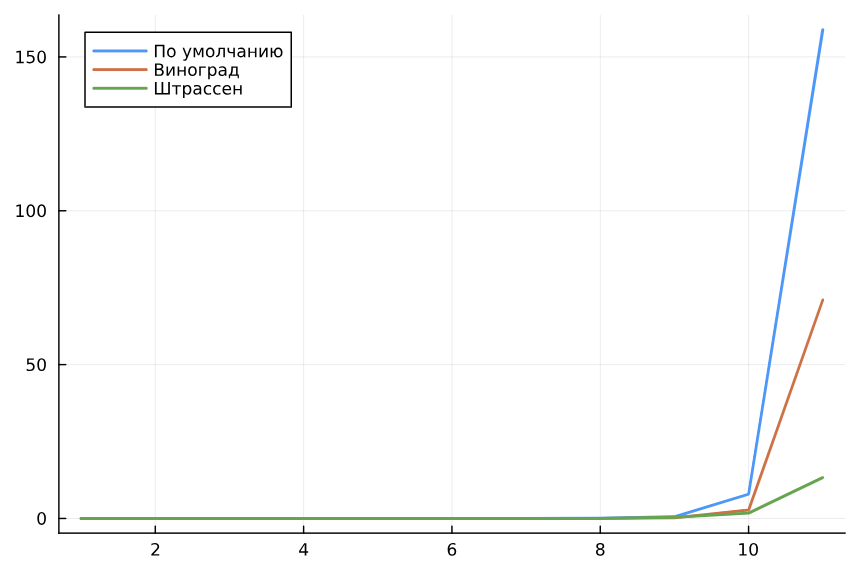
\includegraphics[width=0.8\textwidth]{img1}
\caption{Зависимость ошибки от диалонального доминирования для методов}
\label{fig:img1}
\end{figure}

\section{Выводы}\label{Sect::conclusion}

В ходе выполнения лабораторной работы были построены графики зависимости времени вычисления провизведения двух матриц разными алгоритмами от размерности матриц. Проанализировав графики можно следать вывод о том, что алгоритм Винограда эффективнее классического, а алгоритм Штрассена является наиобее эффективным среди реализованных в рамках данной лабораторной работы.

\end{document}
